\section{实验环境建立}
\subsection{Linux下Clion安装(5分)}
Clion运行界面截图:编译、运行hellolinux.c

\begin{figure}[H]
	\centering
	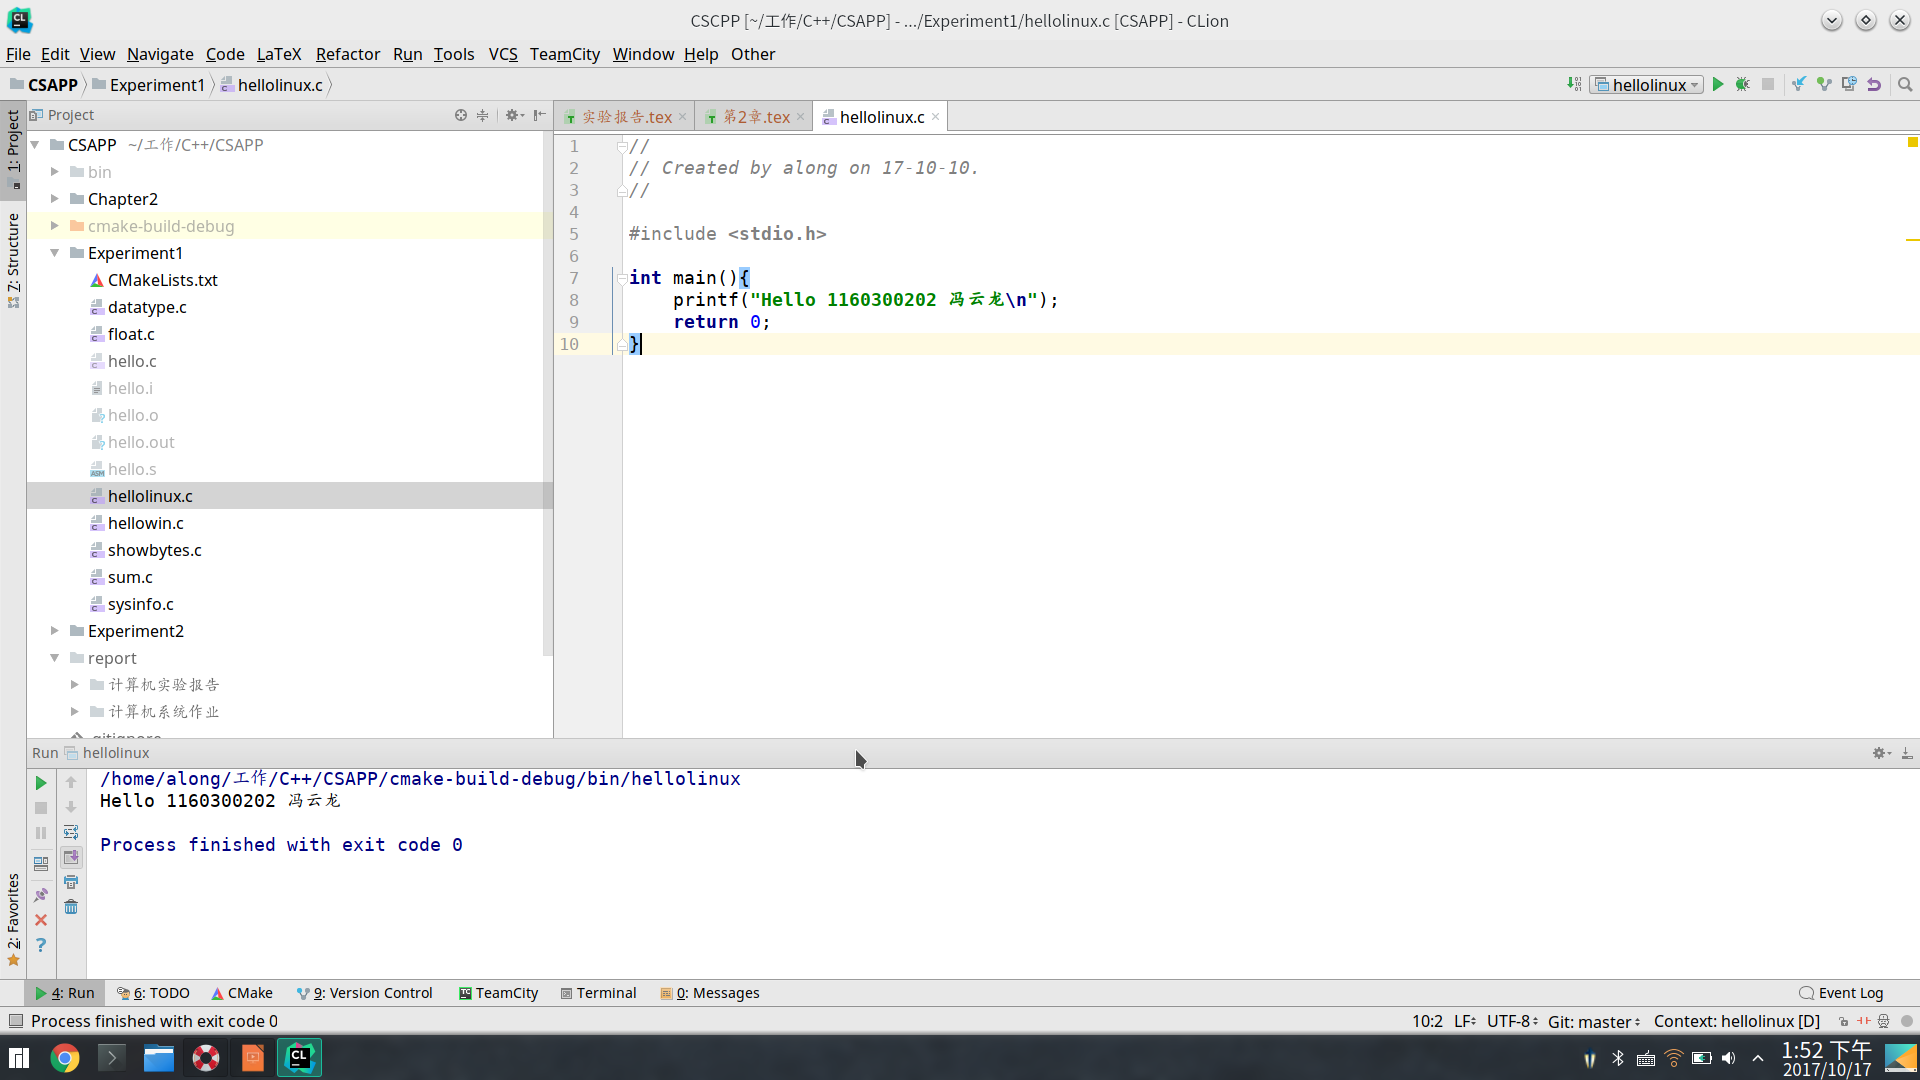
\includegraphics[width=0.55\linewidth]{figures/Linux-Clion}
	\caption{Linux下CLion截图}
	\label{fig:linux-clion}
\end{figure}

\subsection{64位Ubuntu下32位运行环境建立(5分)}

在终端下,用gcc的32位模式编译生成hellolinux.c。执行此文件。
Linux及终端的截图。

\begin{figure}[H]
	\centering
	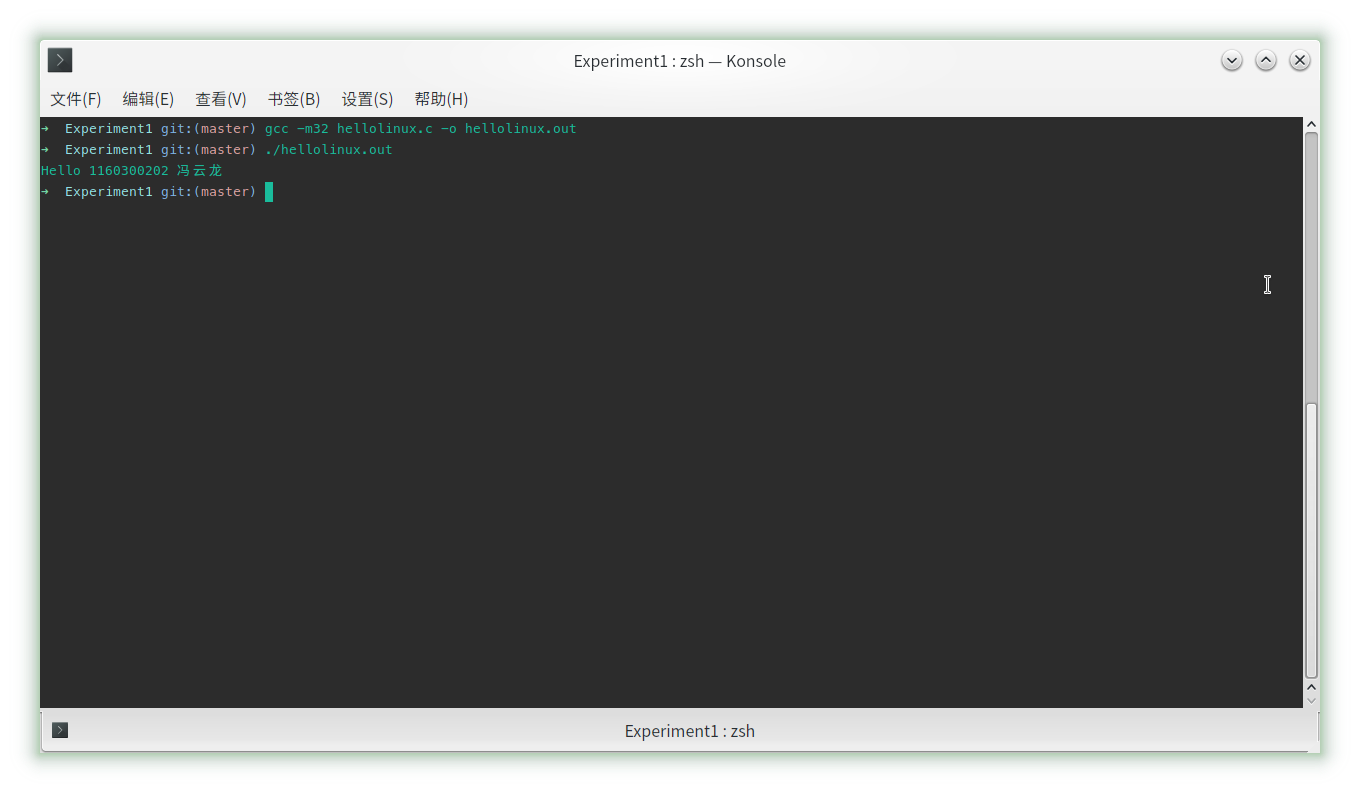
\includegraphics[width=0.5\linewidth]{figures/hello-m32}
	\caption{32位运行环境建立}
	\label{hello-m32}
\end{figure}

